\documentclass[11pt]{article}

\usepackage[ngerman]{babel}
\usepackage[utf8]{inputenc}
\usepackage[T1]{fontenc}%
\usepackage{multirow}
\usepackage{mathtools}
\usepackage{amssymb}
\usepackage{amsfonts}
\usepackage{amsthm}
\usepackage{amsmath}
\usepackage{tabularx}
\usepackage{listings}
\usepackage{textcomp}
\usepackage{tikz-cd}
\usepackage{tikz}
\usepackage{hyperref}
\usepackage{varioref}
\usepackage{pdfpages}
\usepackage{float}

\usetikzlibrary{quotes,babel,arrows,automata,positioning,trees,graphs,shapes,calc,decorations.pathreplacing}

%\theoremstyle{definition}
\newtheorem{definition}{Definition}[section]

\newtheorem{lemma}{Lemma}[section]
\newtheorem{theorem}{Satz}[section]

\theoremstyle{remark}
\newtheorem{example}{Beispiel}
\theoremstyle{corollary}
\newtheorem{corollary}{Korollar}[section]


\newcommand{\tief}[1]{\textsubscript{#1}}
\newcommand{\hoch}[1]{\textsuperscript{#1}}
\newcommand{\sectionbreak}{\clearpage}
\pagestyle{headings}



\author{Jonas Kremer}
\title{Operatorpräzedenzsprachen und ihre Automaten}
\date{\today{}}

%Zeigt nur die zu bearbeitenden Kapitel an, muss am Ende entfernt werden
%\includeonly{sections/definitionen}

\begin{document}
\begin{titlepage}
\thispagestyle{empty}
    \begin{center}
    \large Bachelorarbeit zum Thema:\\
    \vspace{0.5cm}
    \huge \textbf{\textbf{Operatorpräzedenzsprachen und ihre Automaten}} \\
    \vspace{1cm}
    \normalsize
    vorgelegt am: \today \\
    \vspace{2.5cm}
    \large \textbf{Westfälische Wilhelms-Universität Münster}\\
    \vspace{0.5cm} 
    Institut für Informatik
    \vspace{2cm}
    \end{center}
 \normalsize{
    \begin{tabular}{ll}
    	Name: & Jonas Kremer \\
    	Matrikelnummer: & 430666 \\
    	Email: & j\_krem04@uni-muenster.de \\
    	Studiengang: & Bsc. Informatik\\
    	Fachsemester: & 7 (WS. 18/19)\\
    	Arbeitsgruppe: & Softwareentwicklung und Verifikation \\
      	Erstgutachter: & Prof. Dr. Markus Müller-Olm \\
      	Zweitgutachter: & Jens Gutsfeld \\
    \end{tabular}\\
    }
\end{titlepage}

\thispagestyle{empty}
\setcounter{tocdepth}{2}

\tableofcontents
\newpage
\nocite{*}

\section{Motivation}
In dieser Arbeit geht es um die Operatorpräzedenzsprachen (OPL) und um die Eigenschaften ihrer Grammatiken und Automaten. Diese Sprachenklasse wurde 1963 von R.W.Floyd eingeführt, weswegen sie auch häufig als Floydsprachen oder Floydgrammatiken betitelt wird. Floyd interessierte die Struktur von Ausdrücken (sowohl einfache arithmetische als auch programmiertechnische) und die Präzedenz von manchen Operatoren über andere. Besonders interessant war dabei die Präzedenz der Multiplikation über die Addition, die per Konvention gilt und somit nicht explizit durch Klammern verdeutlicht werden muss. Er definiert dafür drei Präzedenzrelationen ($\lessdot, \gtrdot, \doteq$), die zwischen den Terminalsymbolen gelten und in einer Operatorpräzedenzmatrix (OPM) festgehalten werden.\\
Als motivierendes Beispiel, was auch in den Definitionen weiterhin genutzt wird dient ein einfacher arithmetischer Ausdruck mit $\Sigma = \{n, +, \times, (, )\}$:\\ $ n \times (n + n \times n)$, bei dem die implizite Präzedenz deutlich wird.\\
Diese Grammatiken verloren allerdings etwas an Interesse mit der Einführung der LR(k) Parser, was sich erst mit der Entwicklung eines geeigneten äquivalenten Automaten durch Violetta Lonati, Dino Mandrioli und Matteo Pradella im Jahre 2010 änderte. Diese Automaten erkennen exakt die Sprachen, die von den Grammatiken generiert werden und umgekehrt. Die Äquivalenz wird in beide Richtungen gezeigt.
Generell bieten die OPLs viele besondere Eigenschaften: Sie sind eine echte Teilmenge der kontextfreien Sprachen, genießen aber trotzdem alle typischen Abschlusseigenschaften von regulären Sprachen in Bezug auf Boolsche Operatoren, Konkatenation und Kleene-*. 
Weiterhin kann gezeigt werden, dass die Klasse der Visibly-Pushdown Sprachen und Automaten ebenfalls von OPGs und OPAs erkannt werden. Im Gegensatz zu anderen Parsern wie z.B. dem LR(1)- Parser muss hier nicht zwangsläufig von links nach rechts gearbeitet werden, was eine Möglichkeit zur Parallelisierung bietet. Ferner bieten OPLs auch eine Erweiterung zur $\omega- OPL$ und eine \textit{Monadic Second Order Logic Characterization}, was aber den Rahmen dieser Arbeit überschreiten würde.
Als praktischer letzter Teil folgt dann eine Implementierung der OPAs in geeigneter Form.

\section{Vorbereitung und Definitionen}
In diesem Abschnitt geht es um die Definitionen und Namenskonventionen, die für Operatorpräzedenzsprachen benötigt werden. Zunächst kommt eine kurze Definition von kontextfreien Grammatiken, gefolgt von Definitionen und Einschränkungen für Operatorpräzedenzgrammatiken (OPG). Im Anschluss wird die Klasse der Operatorpräzedenzautomaten (OPA) eingeführt, sowohl deterministisch als auch nichtdeterministisch, sowie deren Äquivalenz zu OPGs bewiesen. 
\subsection{Operatorpräzedenzgrammatik}
Eine kontextfreie Grammatik (kfG) ist ein 4-tupel $G = (N, \Sigma, P, S)$, wobei N die Menge der Nichtterminalsymbole, $\Sigma$ die Menge der Terminalsymbole, P die Menge der Produktionsregeln und S das Startsymbol bezeichnet. Folgende Namenskonventionen werden im weiteren Verlauf verwendet: Kleine lateinische Buchstaben am Anfang des Alphabets $a, b, ...$ bezeichnen einzelne Terminalsymbole; Spätere, kleine lateinische Buchstaben $u,v, ...$ bezeichnen Terminalstrings; Große lateinische Buchstaben $A, B, ...$ stehen für Nichtterminalsymbole und griechische Buchstaben $\alpha, \beta, ...$ für beliebige Strings über $N \cup \Sigma$. Sofern nicht explizit eingeschränkt können Strings auch leer sein.\\
Weiterhin haben Produktionsregeln die Form $A \rightarrow \alpha$ mit der \textit{leeren Regel} $A \rightarrow \epsilon$. \textit{Umbenennende} Regeln haben nur ein Nichtterminalsymbol als rechte Seite . Eine \textit{direkte Ableitung} wird mit $\Rightarrow$ beschrieben, eine beliebige Anzahl von Ableitungen mit $\overset{*}{\Rightarrow}$.
\\
Eine Grammatik heisst \textit{reduziert}, wenn jede Regel aus P benutzt werden kann um einen String aus $\Sigma\textsuperscript{*}$ zu erzeugen. Sie ist \textit{invertierbar}, wenn keine zwei Regeln identische rechten Seiten haben.\\
Eine Regel ist in \textit{Operatorform}, wenn ihre rechte Seite keine benachbarten Nichtterminale hat. Entsprechend heisst eine Grammatik, die nur solche Regeln beinhaltet \textit{Operatorgrammatik} (OG). Jede kfG $G=(N,\Sigma, P, S)$ kann in eine äquivalente Operatorgrammatik $G'=(N', \Sigma, P', S)$ umgewandelt werden [siam 25, 38].Die folgenden Definitionen gelten für Operatorpräzedenzgrammatiken (OPGs). \\
\begin{definition}

Für eine OG G und ein Nichtterminal A sinddie \textit{linken und rechten Terminalmengen}  definiert als 
$$ \mathcal{L} \textsubscript{G}(A) = \{ a \in \Sigma | A \overset{*}{\Rightarrow} Ba \alpha \}, \;
 \mathcal{R} \textsubscript{G}(A) = \{ a \in \Sigma | A \overset{*}{\Rightarrow} \alpha aB \}$$
mit $B \in N \cup \{\epsilon\}$
\end{definition}

Auf den Namen der Grammatik G kann verzichtet werden, wenn der Kontext klar ist. Eines der wichtigsten Merkmale von Operatorpräzedenzgrammatiken ist die Definition von drei binären Operatorpräzedenzrelationen.
\begin{definition}[Präzedenzrelationen]\ \\
\label{relationen}
Gleiche Präzedenz: $ a \doteq b \Leftrightarrow \exists A \rightarrow \alpha aBb \beta , 
		B \in N \cup \{ \epsilon \}$ \\
		Übernimmt Präzedenz: $ a \gtrdot b \Leftrightarrow \exists A \rightarrow \alpha Db \beta , D \in N $ and $ a \in
		\mathcal{R}\textsubscript{G}(D)$ \\
		Gibt Präzedenz ab: $ a \lessdot b \Leftrightarrow \exists A \rightarrow \alpha aD \beta , D \in N $ and $ b \in
		\mathcal{L}\textsubscript{G}(D)$
\end{definition}
Es muss beachtet werden, dass diese Relationen im Gegensatz zu ähnlichen arithmetischen Relationen (<,>,=) keine transitiven, symmetrischen oder reflexiven Eigenschaften vorliegen. Weiterhin schließt die Gültigkeit einer Relation die andere nicht aus, sodass zB. sowohl $a \lessdot b$ als auch $a \doteq b$ gelten kann.
Für eine OG G kann eine Operatorpräzedenzmatrix (OPM) $M = OPM(G)$ als $|\Sigma | \times |\Sigma |$ erstell werden, die für jedes geordnete Paar (a,b) die Menge $M \textsubscript{ab}$ der Operatorpräzedenzrelationen beinhaltet. Für solche Matrizen sind Inklusion und Vereinigung natürlich definiert.

\begin{definition}
Eine OG G ist eine OPG oder auch FG gdw. M = OPM(G) eine \textit{konfliktfreie} Matrix ist.\\ 
Also: $\forall a, b, |M \textsubscript{ab} | \leq 1$\\
Eine OPL ist eine Sprache, die durch eine OPG gebildet wird.
\end{definition}

Für solche OPMs werden nun weitere Namenskonventionen vereinbart. Zwei Matrizen sind \textit{kompatibel}, wenn ihre Vereinigung konfliktfrei ist. Eine Matrix heisst \textit{total}, wenn gilt $\forall a, b: M \textsubscript{ab} \neq \emptyset$.
Für eine OPG wird die \textit{Fischer Normalform (FNF)} definiert.

\begin{definition}[Fischernormalform]
Eine OPG G ist in Fischer Normalform gdw. gilt:
\begin{itemize}
\item
G ist invertierbar
\item
G hat keine leeren Regeln außer dem Startsymbol, sofern dies nicht weiter verwendet wird
\item 
G hat keine umbenennenden Regeln
\end{itemize}
\end{definition}

Zu jeder OPG kann eine äquivalente Grammatik in FNF gebildet werden. [ASDFGH]
In Ausblick auf die Operatorpräzedenzautomaten erweitern wir die OPM um ein Symbol $\# \notin \Sigma$, welches Start und Ende eines Strings bezeichnet. Dieses Symbol beeinflusst die Grammatik nicht weiter, da für jedes Terminal gilt: $\forall a \in \Sigma: \# \lessdot a $ und $a \gtrdot \#$. Ferner gilt: $M\textsubscript{\# \#}=\{ \doteq \}$.
\begin{definition}
Ein OP Alphabet ist ein Paar $(\Sigma, M)$ mit:\\
$\Sigma$ ist ein Alphabet \\
M ist eine konfliktfreie OPM, erweitert zu einem $ |\Sigma \cup \{\#\}|\textsuperscript{2}$ Array, das zu jedem geordneten Paar (a,b) höchstens eine OP Relation enthält.
\end{definition} 
Zum Schluss sollte noch eine Einschränkung bezüglich der $\doteq$-Relation getroffen werden. Aus \autoref{relationen} folgt, dass bei einer Regel $A \rightarrow  A \textsubscript{1} a \textsubscript{1}... A \textsubscript{n} a \textsubscript{n} A \textsubscript{n+1}$, bei der alle $A \textsubscript{i}$ potenziell fehlen können, die Relationen $a\textsubscript{1} \doteq a \textsubscript{1} \doteq ... \doteq a \textsubscript{n}$ gebildet werden. Problematisch wird dies, wenn die $\doteq$-Relation \textit{zyklisch} ist dh. es gibt $a\textsubscript{1}, a\textsubscript{2}, ..., a \textsubscript{m} \in \Sigma (m \geq  1)$, sodass $a\textsubscript{1} \doteq a \textsubscript{2} \doteq ... \doteq a \textsubscript{m} \doteq a \textsubscript{1}$. Das führt dazu, dass die Länge der rechten Seite einer Regel keine Begrenzung hat. Wie in meinen Quellen gehe ich auch davon aus, dass die $\doteq$-Relation azyklisch ist. Dies kann einen Einfluss auf die Konstruktion mancher Grammatiken haben, allerdings betrifft es keine der hier verwendeten Grammatiken.\\
Nachdem hier die Grundlagen für die OPGs geschaffen wurden geht es weiter mit den Operatorpräzedenzautomaten.

\subsection{Operatorpräzedenzautomaten}
Die Operatorpräzedenzautomaten(OPA) verhalten sich ähnlich wie Pushdown-Automaten, aber erkennen genau die Operatorpräzedenzsprachen. OPAs arbeiten Bottom-Up, sind aber deutlich einfacher als zB. LR(k) Parser.
\begin{definition}[Operatorpräzedenzautomat]
Ein nichtdeterministischer OPA ist ein 6-Tupel $A=(\Sigma, M, Q, I, F, \delta)$ mit
	\begin{itemize}
	\item
	$(\Sigma, M)$ ist ein OP Alphabet
	\item 
	Q ist eine Menge von Zuständen
	\item
	$I \subseteq Q$ ist die Menge der Startzustände
	\item
	$F \subseteq Q$ ist die Menge der akzeptierenden Zustände
	\item
	$\delta: Q \times (\Sigma \cup Q) \rightarrow \mathcal{P}(Q)$ ist die Übergangsfunktion, die aus drei Teilfunktionen besteht:\\
	$\delta \textsubscript{shift}: Q \times \Sigma \rightarrow \mathcal{P}(Q)$
	$\delta \textsubscript{push}: Q \times \Sigma \rightarrow \mathcal{P}(Q)$
	$\delta \textsubscript{pop}: Q \times Q \rightarrow \mathcal{P}(Q)$
	\end{itemize}
\end{definition}
Wie bei den meisten Automaten, bietet sich auch bei OPAs an eine graphische Darstellung einzuführen. Dabei werden die Zustände als Kreis mit einer Namenskennzeichnung dargestellt. Im weiteren Verlauf der Arbeit werden die Zustände meistens mit $q \textsubscript{i}$, $q \textsubscript{i}$ oder $r \textsubscript{i}$ bezeichnet. \\
Die drei Transitionen werden mit verschiedenen Arten von Pfeilen dargestellt: Ein normaler Pfeil von q nach p mit einem Terminal a als Beschriftung steht für eine Push-Transition $p \in \delta \textsubscript{push}(q, a)$. Ein gestrichelter Pfeil steht für eine Shift-Transition $p \in \delta \textsubscript{shift}(q, a)$. Ein doppelter Pfeil mit einem Zustand r als Beschriftung steht dementsprechend für einen Pop-Move $p \in \delta \textsubscript{pop}(q, r)$\\
Als nächstes wird der Stack des Automaten definiert. Für die Elemente des Stacks definieren wir $\Gamma = \Sigma \times Q$ und erweitern dies um das Symbol für den leeren Stack $\Gamma ' = \Gamma \cup \{\bot\}$. Elemente von $\Gamma'$ haben die Form $\left[a, q\right]$ oder $\bot$.\\
Für $\Gamma ' $ werden ein paar Hilfsfunktionen einegführt: $symbol(\left[ a, q \right]) = a$, $symbol(\bot) = \#$ und $state(\left[ a, q \right]) = q$. Der Stack ist ein String der Form $\Pi = \bot \pi \textsubscript{1} \pi \textsubscript{2}... pi\textsubscript{n}$ mit $\pi\textsubscript{i}\in \Gamma$. Die symbol-Funktion wird auf Strings erweitert, indem das Symbol des letzten Elements ausgegeben wird: $symbol(\Pi)=symbol(\pi \textsubscript{n})$.\\
Eine \textit{Konfiguration} eines OPA ist ein Tripel $C = (\Pi, q, w)$, wobei $\Pi \in \bot \Gamma \textsuperscript{*}$ den aktuelle Stack, $q \in Q$ den Zustand und $w \in \Sigma\textsuperscript{*}\#$ das (übrige) Eingabewort bezeichnet.\\
Bei einem \textit{Lauf} des Automaten handelt es sich um eine endliche Folge von Transitionen/Moves $C\textsubscript{1} \vdash C\textsubscript{2}$. 
\begin{definition}[Übergangsfunktionen]\ Die drei verschiedenen Moves sind wie folgt definiert: \\[1ex]
push move: if $symbol(\Pi) \lessdot a $ then $ (\Pi, p, ax) \vdash (\Pi\left[a, p \right], q, x)$ mit $q \in \delta\textsubscript{push}(p,a)$\\[0.5ex]  
push move: if $a \doteq b $ then $ (\Pi\left[a, p \right], q, bx) \vdash (\Pi\left[b, p \right], r, x)$ mit $r \in \delta \textsubscript{shift}(q,b)$\\[0.5ex]
pop move: if $a \gtrdot b $ then $ (\Pi\left[a, p \right], q, bx) \vdash (\Pi, r, bx)$ mit $r \in \delta \textsubscript{pop}(q,p)$
\end{definition}
Einfach gesagt bedeutet das: Bei einem Push-Move wird der Stack aufgebaut, während das Eingabewort weiter verbraucht wird. Der Shift-Move verarbeitet ebenfalls das Eingabewort, tauscht allerdings nur das Symbol im vorderen Stackelement aus. Der Pop-Move arbeitet dann den Stack ab. Shift- und Pop-Moves werden bei einem leeren Stack nicht ausgeführt.\\
Um den Automaten zu vervollständigen muss die akzeptierte Sprache definiert werden. Eine Konfiguration $(\bot, q\textsubscript{I}, w\#)$ mit $q\textsubscript{I} \ in I$ heisst \textit{initial} und eine Konfiguration $(\bot, q\textsubscript{F}, \#)$ mit $q\textsubscript{F} \in F$ heisst akzeptierend.
\begin{definition}[Akzeptanz der Sprache]
Die Sprache, die von einem OPA A erkannt wird ist definiert als\\
$L(A)=  \Big \{ w | (\bot, q\textsubscript{I}, w\#) \overset{*}{\vdash} (\bot, q \textsubscript{F},\#), q\textsubscript{I} \in I, q \textsubscript{F} \in F \Big \}$
\end{definition}
Damit ist die Definition eines nichtdeterministischen OPAs vollständig.
\subsubsection{Weitere Strukturen}
Um das Verhalten von OPAs beschreiben zu können und die interessanteren Eigenschaften zu beweisen müssen allerdings noch ein paar weitere Grundlagen von OPAs benannt und definiert werden.

\begin{definition}[Einfache Ketten]
Sei ($\Sigma$, M) ein Präzedenz-Alphabet. Eine einfache Kette ist ein Wort $a\tief{0} a\tief{1}a\tief{2}...a\tief{n}a\tief{n+1}$, welches wir als $\hoch{a\tief{0}} \big[ a\tief{1} a\tief{2}... a\tief{n} \big] \hoch{a \tief{n+1}}$ notieren,
mit $a\tief{0}, a\tief{n+1} \in \Sigma \cup \{ \# \}, a\tief{i} \in \Sigma$ für $ 1 \leq i \leq n, M\tief{a\tief{0} a\tief{n+1}} \neq \emptyset$ und $ a\tief{0} \lessdot a\tief{1} \doteq a\tief{2}...a\tief{n} \gtrdot a\tief{n+1}$
\end{definition}

\begin{definition}[Zusammengesetzte Ketten]
Sei ($\Sigma$, M) ein Präzedenz-Alphabet. Eine zusammengesetzte Kette ist ein Wort $a\tief{0} x\tief{0} a\tief{1} x\tief{1} a\tief{2}...a\tief{n}x\tief{n} a\tief{n+1}$ mit $x\tief{i} \in \Sigma \hoch{*}$, bei dem $\hoch{a\tief{0}} \big[ a\tief{1} a\tief{2}... a\tief{n} \big] \hoch{a \tief{n+1}}$ eine einfache Kette ist und jedes $x\tief{i}$ entweder leer$(\epsilon)$ oder wieder eine (einfache oder zusammengesetzte) Kette ist.\\
Die Schreibweise ist $\hoch{a\tief{0}} \big[x\tief{0} a\tief{1} x\tief{1} a\tief{2}... a\tief{n} x\tief{n} \big] \hoch{a \tief{n+1}}$
\end{definition}

Für diese Strukturen benennt man weitere Eigenschaften. Bei einer Kette $\hoch{a} \big[ x \big] \hoch b$ wird x der \textit{Rumpf} genannt. Die \textit{Tiefe} d(x) einer Kette wird rekursiv definiert: $d(x) = 1$, wenn x eine einfache Kette ist und $d(x\tief{0}a\tief{1} x\tief{1}...a\tief{n} x\tief{n}) = \underset{i}{max}(d(x\tief{i})) + 1$ bei zusammengesetzten Ketten. Die Struktur der Ketten ist gleich der internen Struktur von Eingabewörtern und so kann die Tiefe einfach abgelesen werden, wenn ein Syntaxbaum gebildet wird. Die Tiefe einer Kette ist gleich der Tiefe des Rumpfes. Bei der Handhabung von zusammengesetzten Ketten ist es sinnvoll die Rümpfe mit Variablen abzukürzen.\\
Mit diesen Ketten lässt sich jetzt die Kompatibilät eines Wortes w mit einer OPM M definieren, die allerdings nicht mit der Akzeptanz für einen OPA verwechselt werden darf.
\begin{definition}[Kompatibilität mit OPM]
Ein Wort w über $(\Sigma, M)$ ist kompatibel mit M, wenn die beiden Bedingungen gelten:
\begin{itemize}
\item
Für jedes aufeinanderfolgende Paar von Nichtterminalen b,c in w muss $M\tief{bc}\neq \emptyset$ gelten
\item
Für jeden Substring x von $\# w\#$ mit $x=a\tief{0}x\tief{0}a\tief{1}x\tief{1}a\tief{2}...a\tief{n}x\tief{n}a\tief{n}$ gilt: Wenn $a\tief{0} \lessdot a\tief{1} \doteq a\tief{2}...a\tief{n-1} \doteq a\tief{n} \gtrdot a\tief{n+1}$ und für alle $0 \leq i \leq n$ ist $x\tief{i}$ entweder $\epsilon$ oder $\hoch{a\tief{i}} \left[ x \right] \hoch{a\tief{n+1}}$ ist eine Kette, dann ist $M\tief{a\tief{0}a\tief{n+1}} \neq \emptyset$
\end{itemize}
\end{definition}

\subsection{Deterministischer vs. Nichtdeterminstischer OPA}
\subsection{Äquivalenz von OPG und OPA}


\section{(Abschluss-) Eigenschaften von OPLs}
In diesem Abschnitt geht es um die wichtigsten Eigenschaften von Operatorpräzedenzautomaten, wie die Äquivalenz zwischen OPG und OPA, der Äquivalenz von deterministischen und nichtdeterministischen OPAs und den Abschlusseigenschaften, sowie eine Einordnung von anderen Automatenklassen wie endliche Automaten und Visibly-Pushdown Automaten. Weiterhin werden zu allen Eigenschaften die Beweise geführt.
\subsection{Äquivalenz von OPG und OPA}
Eine wesentliche Eigenschaft vieler Sprachklassen ist die Äquivalenz ihrer Grammatiken mit den Automaten. Mit dem vorgestellten OPA haben die OPL nun einen Automaten, der genau die Grammatik erkennt. Die Äquivalenz wird in beiden Richtungen gezeigt.

\subsubsection{Von OPGs zu OPAs}
\begin{lemma}
Sei $G=(N,\Sigma, P, S)$ eine OPG. Dann kann ein OPA A konstruiert werden, sodass $L(G)=L(A)$. Weiterhin sei m die Summer der rechten Seite von Produktionsregeln in G. Dann hat A $O(m^2)$ Zustände.
\end{lemma}
\begin{proof}
Zunächst wird der nichtdeterministische OPA $A=(\Sigma, M, Q, I,F, \delta)$ aus einer gegebenen Grammatik mit derselben OPM konstruiert.\\
Ohne Beschränkung der Allgemeinheit wird angenommen, dass die Grammatik G keine leeren oder umbenennenden Regeln hat. Der OPA A wird nun so konstruiert, dass eine akzeptierende Berechnung dem Aufbauen eines Bottom-Up Ableitungsbaums in G gleicht. Der Automat führt eine Pushtransition aus, wenn das erste Terminal einer neuen rechten Regelseite gelesen wird. Eine Shift-transition  wird ausgeführt bei Terminalsymbolen innerhalb der rechten Seite einer Regel und schätzt nichtdeterministisch das Nichtterminal der linken Seite. Jeder Zustand enthält dabei zwei Informationen: Die erste Komponente repräsentiert dabei das Präfix der rechten Seite unter Konstruktion, während die zweite genutzt wird um die rechte Seite, die vorher unter Konstruktion war, wiederherzustellen, wenn alle verschachtelten rechten Seiten fertiggestellt wurden.\\
Genau definiert wird die Konstruktion folgendermaßen: Sei \\
\centering
$\mathbb{P}={\alpha\in (N\cup\Sigma)*\Sigma|\exists a\rightarrow\alpha\beta\in P}$
die Menge der Präfixe, die auf ein Terminalsymbol enden, der rechten Regelseiten in G. Weiter sei\\
\centering
$\mathbb{Q}=\{\epsilon\}\cup\mathbb{P}\cup N$,\\
$Q=\mathbb{Q} \times (\{\epsilon\} \cup \mathbb{P})$, $I={(\epsilon, \epsilon)}$ und $F=S\times \{\epsilon\} \cup \{(\epsilon, \epsilon|\epsilon\in L(G)\}$
Anmerkung: $|\mathbb{Q}|=1+|\mathbb{P}|+|N|$ ist $O(m)$, also hat Q $O(m^2)$ Zustände\\
Die Transitionen sind folgendermaßen definiert für $a\in \Sigma, \quad \alpha, \alpha_1, \alpha_2\in\mathbb{Q}$ und $\beta, \beta_1, \beta_2 \in \mathbb{P} \cup \{\epsilon\}$:
\begin{itemize}
\item
$\delta_{push}\big ( (\alpha, \beta),a \big )\ni 
\begin{cases}
(a, \alpha) & if; \alpha \notin N, \\
(\alpha a, \beta) & if;  \alpha \in N, \\
\end{cases}$
\item
$\delta_{shift}\big ( (\alpha, \beta),a \big )\ni 
\begin{cases}
(\alpha a, \beta) & if; \alpha \notin N, \\
(\beta\alpha a, \beta) & if;  \alpha \in N, \\
\end{cases}$
\item
$\delta_{pop}\big ( (\alpha_1, \beta_1), (\alpha_2, \beta_2) \big ) \ni (A, \gamma)$, für jedes A, sodass\\
$\begin{cases}
A\rightarrow \alpha_1\in P & if; \alpha_1 \notin N,\\
A\rightarrow \beta_1\alpha_1 \in P & if; \alpha_1 \in N,\\
\end{cases}$ und $\gamma= 
\begin{cases}
\alpha_2 & if; \alpha_2 \notin N, \\
\beta_2 & if; \beta_2 \in N. \\
\end{cases}$
\end{itemize}
\end{proof}



\subsection{Deterministischer vs. Nichtdeterminstischer OPA}
Die vorherige Definition von OPAs war nichtdeterministisch. Eine vorteilhafte Eigenschaft von OPAs ist nun die Äquivalenz der deterministischen und nichtdeterministischen Version. Dadurch unterscheidet sich diese Familie der Automaten wesentlich von den Kellerautomaten. \\
In diesem Abschnitt geht es um die Definition und die Konstruktion eines solchen deterministischen OPAs und um die Lemmata, die nötig sind um die Korrektheit zu beweisen.
\begin{definition}[Deterministischer OPA]
Ein OPA $A=(\Sigma, M, Q, I, F, \delta)$ ist deterministisch, wenn gilt:
\begin{itemize}
\item
I besteht aus nur einem Element \footnote{Hier wird nicht zwischen einem einzelnen Element und einer Menge mit nur einem Element unterschieden.}
\item
$\delta: Q \times \{Q \cup \Sigma\} \rightarrow Q\}$ \\
($\delta$ bildet auf Q ab, anstatt auf $\mathcal{P}(Q)$)
\end{itemize}
\end{definition}
Bei der Konstruktion eines deterministischen OPA aus einem nichtdeterministischen wird folgende Grundidee verwendet: Es muss sichergestellt werden, dass die Pop-Moves von verschiedene Läufen des nichtdeterministischen Automaten nicht mit falschen initialen und finalen Zuständen vermischt werden. Dazu werden Informationen zu dem Pfad, die der Automat seit dem Push-Move, also dem Beginn einer Kette, genommen hat, gesammelt. Dazu wird jeder Zustand des deterministischen Automaten als Menge von Zustandspaaren defininiert. Der deterministische Automat simuliert den nichtdeterministischen Lauf mithilfe des ersten Zustand des Paares und speichert den Zustand, von dem aus der Push-Move ausging im zweiten Zustand. Die deterministischen Pop-Moves werden anhand  der nichtdeterministischen Pop-Moves die für den ersten Zustand und dem Zustand, der vor dem letzten Push-Move erreicht wurde (Was dem obersten Stackeintrag entspricht), definiert sind simuliert.\\
Das wird nun in einem Lemma formal ausgedrückt und bewiesen.
\begin{lemma}
\label{lemma_Deter}
Aus einem nichtdeterminischen OPA A mit s Zuständen kann ein äquivalenter deterministischer OPA $\tilde{A}$ mit $2^{O(s^2)}$ Zuständen konstruiert werden.
\end{lemma}
\begin{proof}
Sei $A=(\Sigma, M, Q, I, F, \delta)$ ein nichtdeterministischer OPA. Der deterministsiche OPA $\tilde{A}=(\Sigma, M, \tilde{Q}, \tilde{I}, \tilde{F}, \tilde{\delta}$ wird wie folgt definiert:
\begin{itemize}
\item
$\tilde{Q} = \mathcal{P}(Q \times (Q \cup \{\top\}))$, wobei $\top \notin Q$ für den Basis der Berechnungen (leerer Stack) steht. \footnote{Zustände in $\tilde{Q}$ werden mit K bezeichnet}
\item
$\tilde{I}=I\times \{\top \}$ ist der Startzustand
\item
$\tilde{F}=\left\{K|K \cap (F \times \{\top\}) \neq \emptyset\right\}$
\item
$\tilde{\delta}: \tilde{Q} \times (\Sigma \cup \tilde{Q})\rightarrow \tilde{Q}$ ist die Übergangsfunktion ist die Vereinigung aus den drei Teilfunktionen:\\[2ex]
$\tilde{\delta}_{push}: \tilde{Q} \times \Sigma \rightarrow \tilde{Q}$ ist definiert als: 
\begin{equation*}
\tilde{\delta}_{push}(K, a) = \bigcup\limits_{(q,p) \in K} \{(h,q)|h \in \delta_{push}(q,a)\}
\end{equation*}
$\tilde{\delta}_{shift}: \tilde{Q} \times \Sigma \rightarrow \tilde{Q}$ ist definiert als: 
\begin{equation*}
\tilde{\delta}_{shift}(K, a) = \bigcup\limits_{(q,p) \in K} \{(h,p)|h \in \delta_{shift}(q,a)\}
\end{equation*}
$\tilde{\delta}_{pop}: \tilde{Q} \times \tilde{Q}\rightarrow \tilde{Q}$ ist definiert als: 
\begin{equation*}
\tilde{\delta}_{pop}(K_1, K_2) = \bigcup\limits_{(r,q) \in K_1, (q,p)\in K_2} \{(h,p)|h \in \delta_{pop}(r,q)\}
\end{equation*}
\end{itemize}
Die Zahl s der Zustände wächste exponential: Sei s = $|Q|$ die Anzahl der Zustände vom nichtdeterministischen Automaten A, dann ist $|\tilde{Q}| = 2^{|Q| * |Q \cup \{\top\}|}$. Also hat $\tilde{A}$ genau $2^{O(s^2)}$ Zustände.\\
Die Äquivalenz der beiden Automaten basiert auf den Aussagen der beiden folgenden Lemmata, die in jeweils Richtungen zeigen, dass äquivalente Supports gebildet werden:
\begin{lemma}
Sei y der Rumpf einer Kette mit der Stütze $q\stackrel{y}{\rightsquigarrow} q^\prime$ in A. Dann gilt für alle $p \in Q$ und $K \in \tilde{Q}$, wenn $(q,p) \in K$, dann existiert eine Stütze $K\stackrel{y}{\rightsquigarrow} K^\prime$ mit $(q^\prime, p) \in K^\prime $
\end{lemma}
\begin{proof}
\label{lemma_deter1}
Beweis durch Induktion der Tiefe h = $d(y)$. 
\paragraph{Induktionsanfang: (h = 1)}\ \\
Wenn h = 1 ist, dann ist $y = a_1a_2...a_n$ und die Stütze in A hat die Form $q  \stackrel{a_1}{\rightarrow} q_1 \dashrightarrow ... \dashrightarrow q_{n-1} \stackrel{a_n}{\dashrightarrow} q_n \stackrel {q_0} {\Rightarrow} q^\prime$.\\[1,5ex] Sei \\[1ex]
\begin{tabular}[c]{l}
$K_1=\tilde{\delta}_{push}(K, a_1)$,\\
$K_i=\tilde{\delta}_{shift}(K_{i-1}, a_1)\quad$, für jedes $i=2,...,n$\\
$K^\prime = \tilde{\delta}_{pop}(K_n, K)$.
\end{tabular}
\\[1,5ex]Dann ist
\begin{equation*}
K\stackrel{a_1}{\rightarrow} K_1 \stackrel{a_2}{\dashrightarrow} ... \stackrel{a_{n-1}}{\dashrightarrow} K_{n-1} \stackrel{a_n}{\dashrightarrow} K_n \stackrel {q_0} {\Rightarrow} K^\prime. 
\end{equation*}
die Stütze in $\tilde{A}$. Weiterhin gilt für $(q,p) \in K$ aufgrund der Definition von $\tilde{\delta}$:\\
\begin{tabular}{l l}
$(q_1,q) \in K_1$, & da $q_1 \in \delta_{push}(q, a_1)$, \\
$(q_i, q) \in K_i$, & da $q_i \in \delta_{shift}(q_{i-1})$, \\
$(q^\prime, p) \in K^\prime$, & da $q^\prime \in \delta_{pop}(q_n, q)$ 
\end{tabular}
\paragraph{Induktionsschritt}\ \\
Nun gelte Induktionsannahme für Stützen mit einer geringeren Tiefe als h. Weiter sei $y = x_0a_1x_1a_2...a_nx_n$ mit der Tiefe h und der Stütze $q \stackrel{x_0}{\rightsquigarrow} q_0^{\prime} \stackrel{a_1}{\rightarrow} q_1\stackrel{x_1}{\rightsquigarrow} q_1^{\prime} \dashrightarrow ... \dashrightarrow q_{n-1} \stackrel{a_n}{\dashrightarrow} q_n \stackrel{x_n}{\rightsquigarrow} q_n^{\prime} \stackrel {q_0^{\prime}} {\Rightarrow} q^\prime$, wobei $q_i^\prime = q_i$, wenn $x_i = \epsilon$ und jedes nichtleere $x_i$ hat eine geringere Tiefe als h. Dann kann man aufgrund der Induktionsannahme und der Definition von $\tilde{\delta}$ eine Stütze
\begin{eqnarray*}
K \stackrel{x_0}{\rightsquigarrow} K_0^{\prime} \stackrel{a_1}{\rightarrow} K_1\stackrel{x_1}{\rightsquigarrow} K_1^{\prime} \dashrightarrow ... \dashrightarrow K_{n-1} \stackrel{a_n}{\dashrightarrow} K_n \stackrel{x_n}{\rightsquigarrow} K_n^{\prime} \stackrel {K_0^{\prime}} {\Rightarrow} K^\prime 
\end{eqnarray*}
konstruieren und weil $(q,p) \in K$ ist, gilt:\\[1ex]
\begin{tabular}[c] {l l}
$(q_0^\prime, p) \in K_0^\prime $  & durch die Induktionsannahme auf die Stütze $q \stackrel{x_0}{\rightsquigarrow} q_0^\prime$ \\
$ (q_1, q_0^\prime) \in K_1$, & denn $q_1 \in \delta_{push}(q_0^\prime, a_1)$ \\
$(q_1^\prime, q_0^\prime) \in K_1^\prime$, & durch die Induktionsannahme auf die Stütze $q_1 \stackrel{x_1}{\rightsquigarrow} q_1^\prime$\\ 
$ (q_i, q_0^\prime) \in K_i$, & denn $q_i \in \delta_{shift}(q_{i-1}^\prime, a_1)$ für jedes $i=2,...,n$ \\
$(q_i^\prime, q_0^\prime) \in K_i^\prime$, & durch die Induktionsannahme auf die Stütze $q_i \stackrel{x_i}{\rightsquigarrow} q_i^\prime$\\ 
$ (q^\prime, p) \in K^\prime$, & denn $q^\prime \in \delta_{pop}(q_n, q_0^\prime)$ \\
\end{tabular}
Und dadurch ist der Beweis abgeschlossen.
\end{proof}
Die Aussage des nächsten Lemmas führt genau anders herum, vom Automaten $\tilde{A}$ zu A.
\begin{lemma}
\label{lemma_deter2}
Sei y der Rumpf einer Kette mit der Stütze $K \stackrel{y}{\rightsquigarrow} K^\prime$ in $\tilde{A}$. Dann gilt für alle $p, q^\prime \in Q$: Wenn $(q^\prime, p) \in K^\prime$, dann existiert eine Stütze $q \stackrel{y}{\rightsquigarrow} q^\prime$ in A.
\end{lemma}
\begin{proof}
Zunächst ein paar Anmerkungen, die für den Beweis verwendet werden:
\renewcommand{\labelenumi}{\roman{enumi})}
\begin{enumerate}
\item
Aus der Definition von $\delta_{push}$ folgt: Wenn es $\bar{K} \stackrel{a}{\rightarrow} K$ in $\tilde{A}$ gibt mit $(\bar{q}, q) \in K, \quad (q,p) \in \bar{K}$, dann gibt es $q \stackrel{a}{\rightarrow} \bar{q}$ in A.
\label{rem1}
\item
Aus der Definition von $\delta_{shift}$ folgt: Wenn es $\bar{K} \stackrel{a}{\dashrightarrow} K$ in $\tilde{A}$ gibt mit $(r,q) \in K$, dann existiert ein $\bar{q} \in Q$, sodass $\bar{q} \stackrel{a}{\dashrightarrow} r$ in A und $(\bar{q}, q) \in K$.
\label{rem2}
\item
Aus der Definition von $\delta_{pop}$ folgt: Wenn es $\bar{K} \stackrel{K}{\Rightarrow} K$ in $\tilde{A}$ gibt mit $(q^\prime q) \in \bar{K}$, dann existiert ein Paar $(r,q) \in \bar{K}$, sodass $(q,p)\in K$ und es gibt $r \stackrel{q}{\Rightarrow} q^\prime$ in A.
\label{rem3}
\end{enumerate}

Beweis durch Induktion auf die Höhe $h=d(y)$ 
\paragraph*{Induktionsanfang: (h=1)}
Wenn h=1 ist, dann ist $y=a_1a_2...a_n$ mit der Stütze $K\stackrel{a_1}{\rightarrow} K_1 \stackrel{a_2}{\dashrightarrow} ... \stackrel{a_{n-1}}{\dashrightarrow} K_{n-1} \stackrel{a_n}{\dashrightarrow} K_n \stackrel {q_0} {\Rightarrow} K^\prime.$ Sei $(q^\prime, p) \in K$, dann gibt es wie in Anmerkung \ref{rem3} in $\tilde{A}$ ein Paar $(q_n, q) \in K$, sodass $(q,p) \in K$ und $q_n \stackrel{q}{\Rightarrow} q^\prime$. Weiterhin folgt aus Anmerkung \ref{rem2} mit $(q_n, q) \in K$ und  $K_{n-1} \stackrel{a_n}{\dashrightarrow} K_n$ die Existenz eines Zustandes $q_{n-1} \in Q$, sodass $(q_n,q) \in K_{n-1}$ und $q_{n-1} \stackrel{a_n}{\dashrightarrow} q_n$. Auf gleiche Weise gilt für alle $i=n-2,...,1$, dass es $q_i \in Q$ gibt, sodass $(q_i,q) \in K_i$ und $q_i \stackrel{a_{i+1}}{\dashrightarrow} q_{i+1}$ Schließlich folgt aufgrund Anmerkung \ref{rem1} aus $K\stackrel{a_1}{\rightarrow} K_1$, $(q_1, q) \in K_1$ und $(q, p) \in K$, dass es $q \stackrel{a_1}{\rightarrow} q_1$ in A gibt. So wurde gezeigt, dass es eine Stütze für y gibt.
\paragraph*{Induktionsschritt} 
Nun gelte die Induktionsannahme für eine geringere Tiefe als h. Weiter sei $y=x_0a_1x_1a_2...a_nx_n$ mit der Tiefe h und der Stütze $K \stackrel{x_0}{\rightsquigarrow} K_0^{\prime} \stackrel{a_1}{\rightarrow} K_1\stackrel{x_1}{\rightsquigarrow} K_1^{\prime} \dashrightarrow ... \dashrightarrow K_{n-1} \stackrel{a_n}{\dashrightarrow} K_n \stackrel{x_n}{\rightsquigarrow} K_n^\prime \stackrel{K_0^{\prime}} {\Rightarrow} K^\prime$, wobei $K_i^\prime = K_i$, wenn $x_i= \epsilon$ und jedes nichtleere $x_i$ hat eine geringere Tiefe als h. Sei $(q^\prime, p) \in K^\prime$. Da es aufgrund von Anmerkung \ref{rem3} $K_n^\prime \stackrel{K_0^\prime} {\Rightarrow} K^\prime$ gibt, existiert ein Paar $(q_n^\prime, q_0^\prime) \in K_n^\prime$ in $\tilde{A}$ mit $(q_0^\prime, p) \in K_0^\prime$ und $q_n^\prime \stackrel{q_0^\prime}{\Rightarrow} q^\prime$. Wenn $x_n \neq \epsilon$ existiert aufgrund der Induktionsannahme, da $(q_n^\prime, q_0^\prime) \in K_n^\prime$, eine Stütze $q_n \stackrel{x_n}{\rightsquigarrow} q_n^\prime$ mit $(q_n, q_0^\prime \in K_n$. Auf gleiche Weise gilt für alle $i=n-1,...2,1$: Es existieren $q_i^\prime$ und $q_i$ ($q_i^\prime=q_i$, wenn $x_i= \epsilon$), sodass es $q_i \stackrel{x_i}{\rightsquigarrow} q_i^\prime \stackrel{a_{i+1}}{\dashrightarrow}q_{i+1}$ in A gibt,

\begin{tabular}{l p{8cm}}
mit $(q_i^\prime, q_0^\prime) \in K_i^\prime$ & (Aufgrund von Anmerkung \ref{rem2}, da $K_i^\prime \stackrel{a_{i+1}}{\dashrightarrow} K_{i+1}$ in $\tilde{A}$ und $(q_{i+1}, q_0^\prime) \in K_{i+1}$)\\

 und $(q_i^\prime, q_0^\prime) \in K_i$ & (Aufgrund der Induktionsannahme, da $K_i \stackrel{x_i}{\rightsquigarrow} K_i^\prime$ in $\tilde{A}$ und $(q_i^\prime, q_0^\prime) \in K_i^\prime$).
  \end{tabular}\\
 Das gilt speziell auch für $q_1 \stackrel{x_1}{q_1^\prime}$ mit $(q_1, q_0^\prime) \in K_1$. Weiterhin gibt es $(q_0^\prime \stackrel{a_1}{\rightarrow} q_1$, da $K_0^\prime \stackrel{a_1} {\rightarrow} K_1$ und $(q_0^\prime, p) \in K_0^\prime$ (Anmerkung \ref{rem1}).
 
 Schließlich folgt aus der Induktionsannahme, da $(q_0^\prime, p) \in K_0^\prime$ und $K\stackrel{x_0}{rightsquigarrow} K_0^\prime$, wenn $x_0 \neq \epsilon$ existiert ein Zustand $q \in Q$, sodass $q \stackrel{x_0}{\rightsquigarrow} q_0^\prime$ in $\tilde{A}$ mit $(q,p) \in K$. Somit haben wir eine Stütze nach \autoref{Support} (2) konstruiert und der Beweis ist abgeschlossen.
  \end{proof}
Um den Beweis von \autoref{lemma_Deter} zu vervollständigen muss noch bewiesen werden, dass eine akzeptierende Berechnung für y in A gibt, dies auch in $\tilde{A}$ zutrifft. 

Sei $y \in L(A)$. Dann gibt es eine Stütze $q \stackrel{y} {\rightsquigarrow} q^\prime$, wobei $q\in I, q^\prime \in F$. Dann folgt aus \autoref{lemma_deter1} für $(q_0, \top) \in K=I \times \{\top\}$, dass eine Stütze $K \stackrel{y}{\rightsquigarrow}K^\prime$ in $\tilde{A}$ mit $(q^\prime, \top) \in K^\prime $. $q^\prime \in F$ impliziert $K^\prime \in F^\prime$
Andersherum sei $y \in L(\tilde{A})$. Dann hat y eine Stütze $\tilde{K}\stackrel{y}{\rightsquigarrow}K^\prime$ in $\tilde{A}$ mit $K^\prime \in \tilde{F}$. Das heißt es existiert ein $q^\prime \in F$, sodass $(q^\prime, \top) \in K^\prime$. Aufgrund von \autoref{lemma_deter2} gibt es eine Stütze $q \stackrel{y} {\rightsquigarrow} q^\prime$ in A mit $(q^\prime, \top) \in \tilde{K}$ und daraus folgt $q \in I$. Somit definiert $q\stackrel{y}{\rightsquigarrow}q^\prime$ eine akzeptierende Berechnung für y in A.
Damit ist der Beweis abgeschlossen. 
\end{proof}
\subsection{Abgeschlossenheit}

\subsection{Visibly Pushdown Sprache als Teilklasse}

\section{Implementierung der OPA}
In diesem Abschnitt geht es um eine Implementierung einer Bibliothek für OPA in einer Programmiersprache. Dazu folgt eine kurze Aufzählung der verwendeten Programme und Ressourcen und anschließend folgt eine Erläuterung zu der Funktionsweise anhand eines Klassendiagramms.
\paragraph*{Verwendete Ressourcen}
Die Bibliothek wurde in der Programmiersprache Java mit dem JDK 1.8 verfasst. Die Sprache Java ist sehr weit verbeitet und sehr gut dokumentiert und vereinfacht strukturiertes und methodisches Vorgehen. Als Umwickelungsumgebung wurde IntelliJ IDEA Ultimate Edition verwendet. Für die Erstellung der Bibliothek  als JAR-Datei und die Verwaltung der Abhängigkeien wurde das Werkzeug Maven der Apache Software Foundation verwendet. Außer den Standardbibliotheken der JDK 1.8 wurde noch \textit{java-tuples} verwendet.

\paragraph*{Design}
Für die Entwickelung wurde hauptsächlich die Definition des OPA direkt in Klassen und Attribute umgesetzt. So besteht zB. die Klasse \textit{OP\_Automat} aus einer Menge von Terminalen (Character), einer OP\_Matrix, einer Menge von Zuständen, der Menge der Start- und Endzustände und einem Objekt der \textit{Transitionen-}Klasse, was der Übergangsfunktion $\delta$ entspricht. Die Präzedenzrelation werden als Enumeration dargestellt. In \autoref{uml1} ist ein vereinfachtes Klassendiagramm für das Paket model.automation dargestellt. 
\begin{figure}
\centering
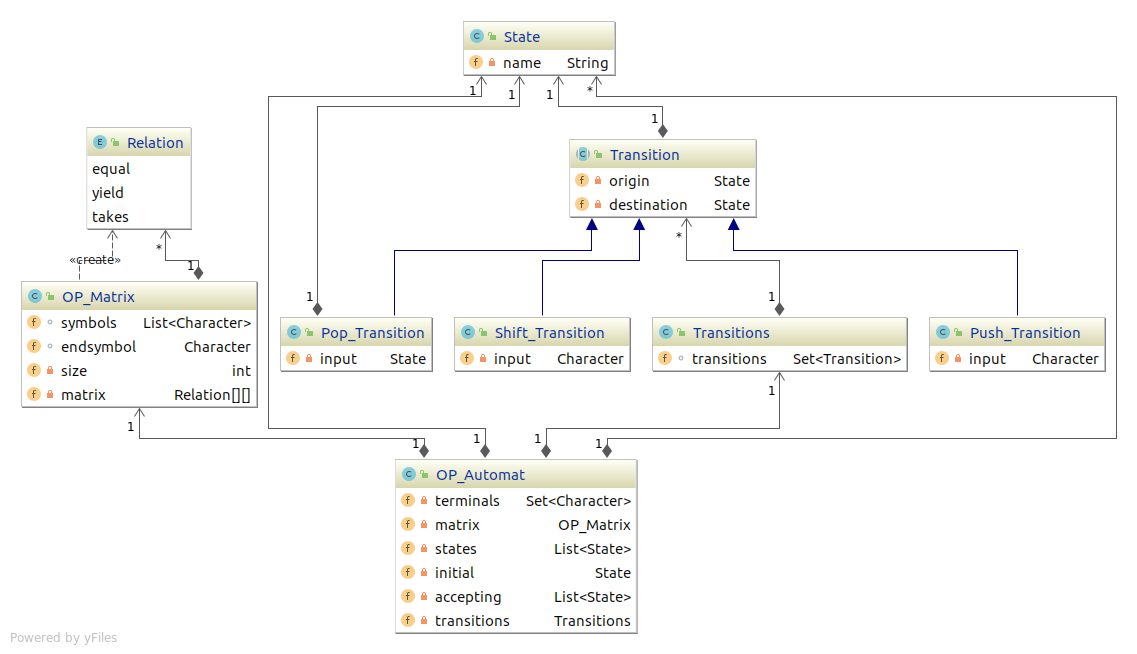
\includegraphics[scale=0.3]{sections/automaton}
\caption{UML Klassendiagramm zum automaton package}
\label{uml1}
\end{figure}
 Wie in den Quellen ist auch hier die Berechnung erst einmal vom reinen Automatenmodell getrennt. Die Berechnung findet in den Klassen des Paketes model.computation statt, welches wie in \autoref{uml2} beschrieben aufgebaut ist. 
 \begin{figure}
 \centering
 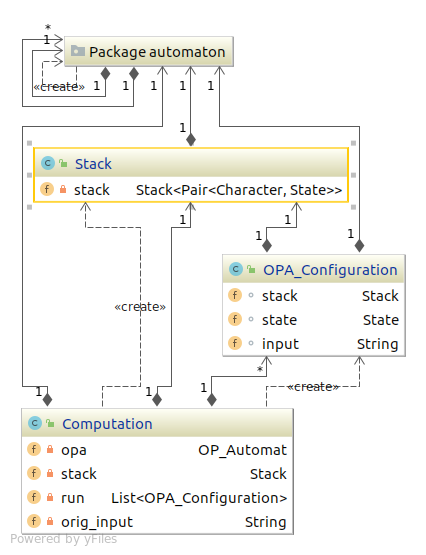
\includegraphics[scale=0.35]{sections/computation}
 \caption{UML Klassendiagramm zum computation package}
 \end{figure}
Um nun eine Berechnung zu starten muss nunächst der Automat initialisiert werden. Dieser besteht aus vielen verschachtelten Attributen, was die Initialisierung sehr aufwendig macht. Es wurde unter anderem durch Verwendung des Builder-Patterns für den Automaten und einer ähnlichen Form für die Matrix und die Transitionen eine etwas komfortablere und intuitivere Nutzung gewährleistet. Dann muss ein Objekt der Klasse \textit{Computation} mit einem OPA und einem Eingabestring erzeugt werden, welches dann durch die \textit{compute} Methode die Berechnung startet und das Ergebnis in der Konsole ausgibt. Um schnelleres Testen zu gewährleisten, wurde ebenfalls eine OPA\_ReaderWriter Klasse erzeugt, die es ermöglicht den Automaten zu serialisieren und somit zu speichern. Das entstandene Format ist dabei allerdings nicht leserlich. Weiterhin wurden zu allen wichtigen Komponenten \textit{print-} Methoden implementiert.\\
Der Automat arbeitet nichtdeterministisch, indem er in jedem Schritt alle möglichen weiteren Schritte berechnet. Am Anfang wird zu jedem initialen Zustand eine Konfiguration erstellt. Es wird immer nur ein Pfad von Konfigurationen bearbeitet bis dieser akzeptiert oder fehlschlägt. An jeder Stelle werden mögliche Alternativen in einer zweiten Warteschlange gespeichert, mit der Information an welcher Stelle diese Alternative einzusetzen ist. Schlägt ein Pfad fehl, wird der Lauf bis zur jüngsten Alternative in der Warteschlange zurückgesetzt und es geht mit der Alternative weiter. Wenn eine akzeptierende Konfiguration erreicht wird, oder keine Alternativen mehr vorhanden sind bei nichtleerem Input, terminiert der Automat. \\
Die Implementierung ist allerdings noch sehr rudimentär und es konnten leider nicht alle Anforderungen erfüllt werden. Es wäre schön gewesen, Konstruktionen für die Abschlusseigenschaften auf Automatenebene zu haben, so konnte lediglich die Vereinigung implementiert werden.

\section{Fazit}
Es war sehr spannend in ein, zwar nicht neues, aber durchaus noch unterrepräsentiertes Thema der Informatik einzutauchen. Ein erneutes Interesse an diesen Sprachen halte ich auf jeden Fall für angebracht. Trotzdem war es eine große Herausforderung in ein so theoretisches Themengebiet einzusteigen und die Definitionen und Beweise zu verinnerlichen. 
In dieser Arbeit wurden die grundlegenden Funktionen und Definitionen der Operatorpräzedenzsprachen zusammengefasst in Hinblick auf die Grammatiken und den Automaten. Weiterhin sind wichtige sprachtheoretische Eigenschaften beleuchtet und bewiesen, sowie in einer praktischen Anwendung implementiert worden. Allerdings gibt es in dem Bereich noch deutlich mehr Potenzial, was in dieser Bachelorarbeit nicht betrachtet wurde, aber zumindest an dieser Stelle als Ausblick erwähnt werden sollte: \begin{itemize}
\item
Eine monadische Prädikatenlogik zweiter Stufe  wurde für die OPL definiert \cite{mso}. 
\item
Die Sprache der OPL wurde erweitert zu $\omega$-OPL für unendliche Wörter. Auch dazu wurde die Prädikatenlogik zweiter Stufe entworfen.\cite{mso}.
\item
Ansätze für ModelChecking von Operatorpräzedenzsprachen \cite{modelchecking}
\item
Weitere Algebraische Eigenschaften der Operatorpräzedenzsprachen \cite{algebraic_properties}
\item
Betrachtung der Sprachen, mit Konflikt in der Matrix
\item
...
\end{itemize}
All das dürfte genügen, damit die Wissenschaft sich noch weiter mit den Operatorpäzedenzsprachen beschäftigen wird und man darf gespannt sein, was in den nächsten Jahren noch an weiteren Ergebnissen folgt. \\
Damit ist die Arbeit abgeschlossen.

\thispagestyle{empty}
\addcontentsline{toc}{section}{Literaturverzeichnis}


\bibliographystyle{unsrt}
\bibliography{sample}
\newpage
\addcontentsline{toc}{section}{Eidesstaatliche Erklärung}
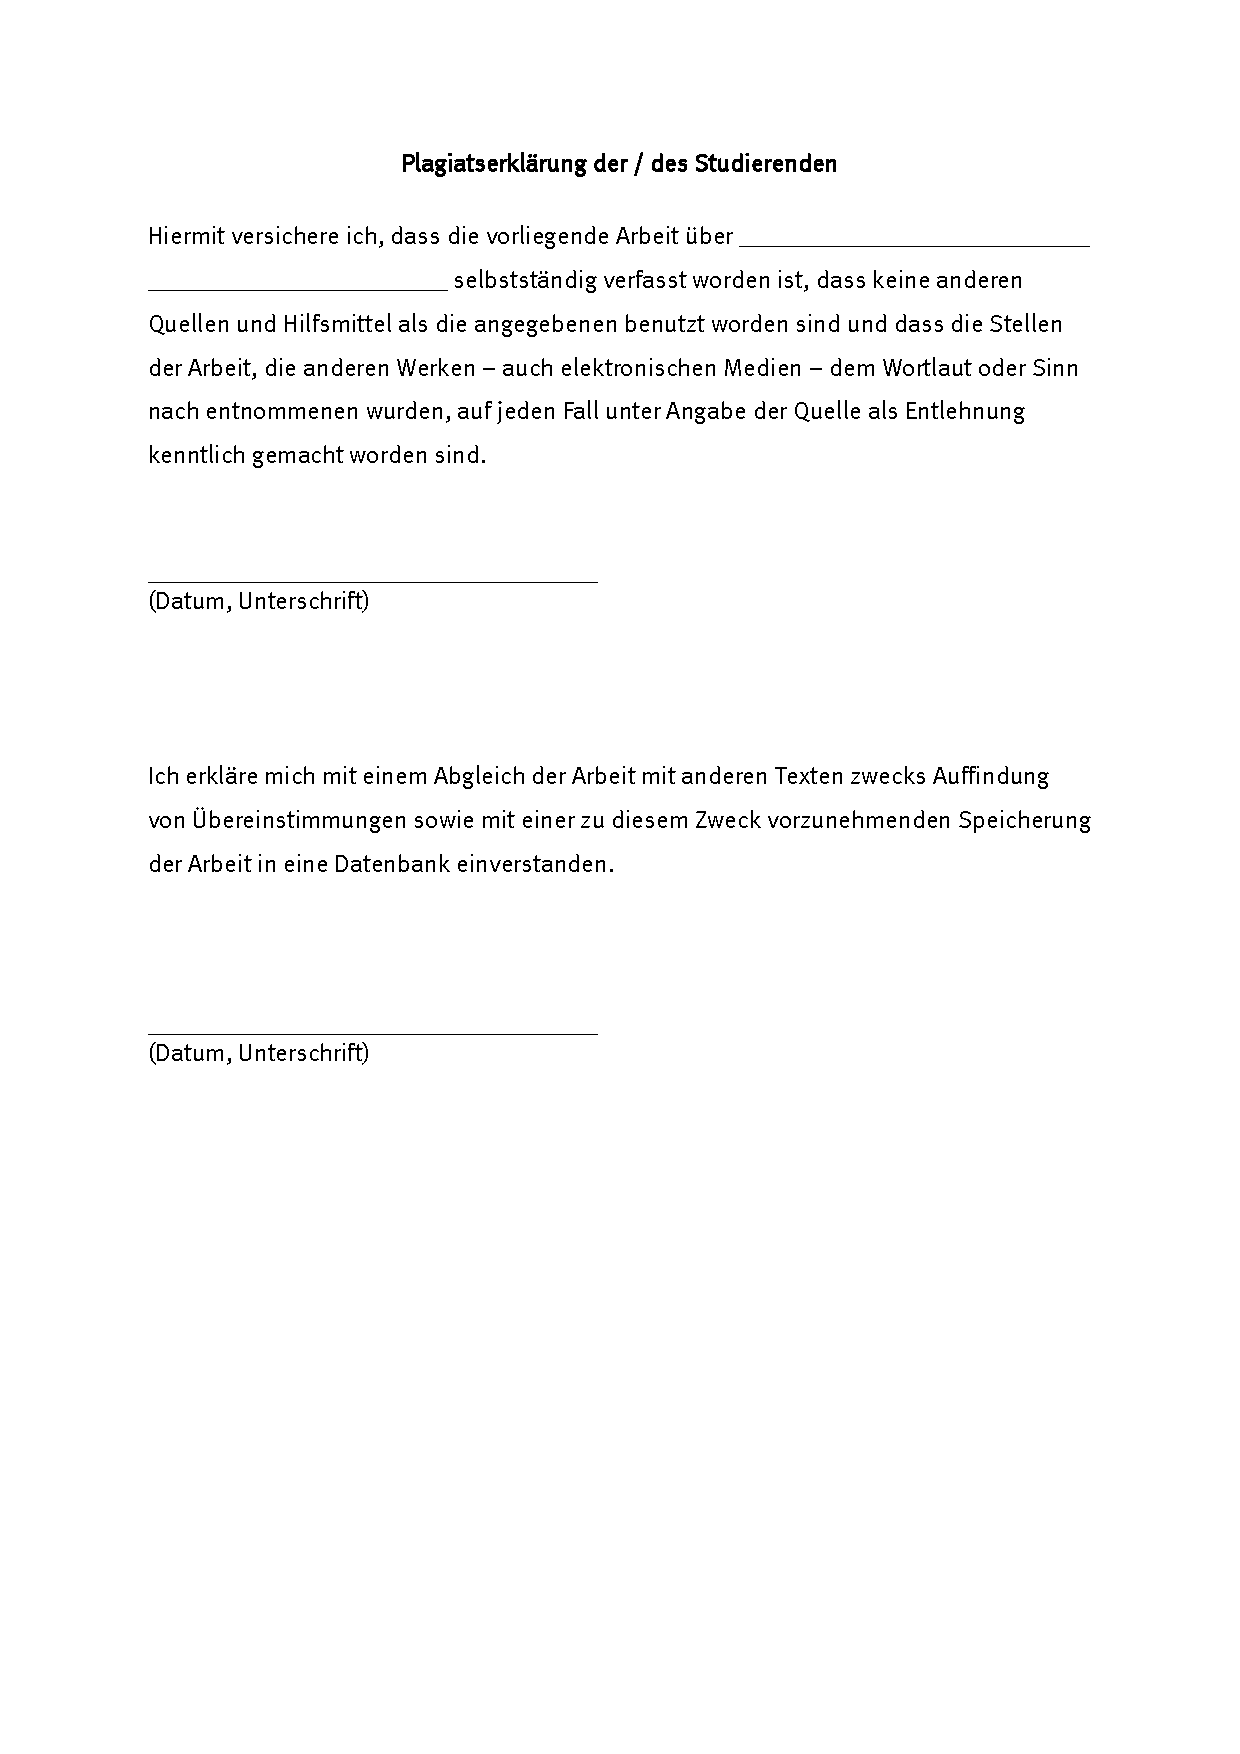
\includepdf{sections/plagiat}


\end{document}